% !TEX encoding = UTF-8
% !TEX TS-program = pdflatex
% !TEX root = ../tesi.tex

%**************************************************************
\chapter{Sportwill}
\label{cap:Sportwill}
%**************************************************************

\intro{In questo capitolo viene descritto il progetto, effettuata un'analisi iniziale dei requisiti per poi definire dettagliatamente come le funzionalità sono state implementate e che tecnologie e strumenti sono stati usati. }\\

%**************************************************************

\section{Descrizione progetto}

\section{Analisi dei requisiti}

\section{Tecnologie e strumenti}

\subsection{Flutter e Dart}

\subsection{Android Studio}

\begin{figure}[htbp]	
	\centering
	
\includegraphics[width=4cm]{immagini/logoandroidstudio.png}
	\caption{Logo Android Studio}
	\label{fig:Logo Android Studio}
\end{figure}

\subsection{GitLab}

\begin{figure}[htbp]	
	\centering
	
\includegraphics[width=4cm]{immagini/logogitlab.png}
	\caption{Logo GitLab}
	\label{fig:Logo GitLab}
\end{figure}

\subsection{Database}

\begin{figure}[htbp]	
	\centering
	
\includegraphics[width=4cm]{immagini/logodbeaver.png}
	\caption{Logo DBeaver}
	\label{fig:Logo DBeaver}
\end{figure}

\subsection{Backend}

\newpage

\section{Implementazioni}

Le implementazioni realizzate durante lo stage sono state: 
\begin{itemize}
	\item Logo;
	\item Filtro di ricerca testo;
	\item Pagina Modifica e campi obbligatori;
	\item Mappa percorso;
	\item Aggiornamento automatico mappa;
	\item Mappa schermo intero;
	\item Colori;
	\item Pagina Modifica;
	\item Eliminazione, Modifica e Aggiunta di un'attività;
	\item Filtro avanzato di ricerca attività.
\end{itemize}
Tutti i servizi sono stati rilasciati su un'apposita repository aziendale su \textit{GitLab}.

\subsection{Logo}
È stato modificato il logo di base di Flutter con quello di Sportwill.\\
Per  fare ciò è stato inserita l'immagine del logo all'interno della seguente cartella \textit{app/src/main/res/mipmap/}.\\

\begin{figure}[htbp]	
	\centering
	
\includegraphics[width=6cm]{immagini/logosportwill.png}
	\caption{Logo Sportwill}
	\label{fig:Logo Sportwill}
\end{figure}

\newpage

\subsection{Filtro di ricerca testo}
All'interno della pagina principale dell'applicazione ovvero la pagina \textit{uscite\_overview\_screen.dart} è stato aggiunto un widget che permette di ricercare le varie card in base all'evento, al luogo o alla persona.\\
Digitando nella barra di ricerca quindi si potranno ricercare solo le card a cui si è interessati.\\
Per fare ciò è stato inserita una funzione chiamata \textit{ricerca()} che ritorna una TextField come Widget nel file \textit{uscite\_overview\_screen.dart}.\\

\begin{figure}[htbp]	
	\centering
	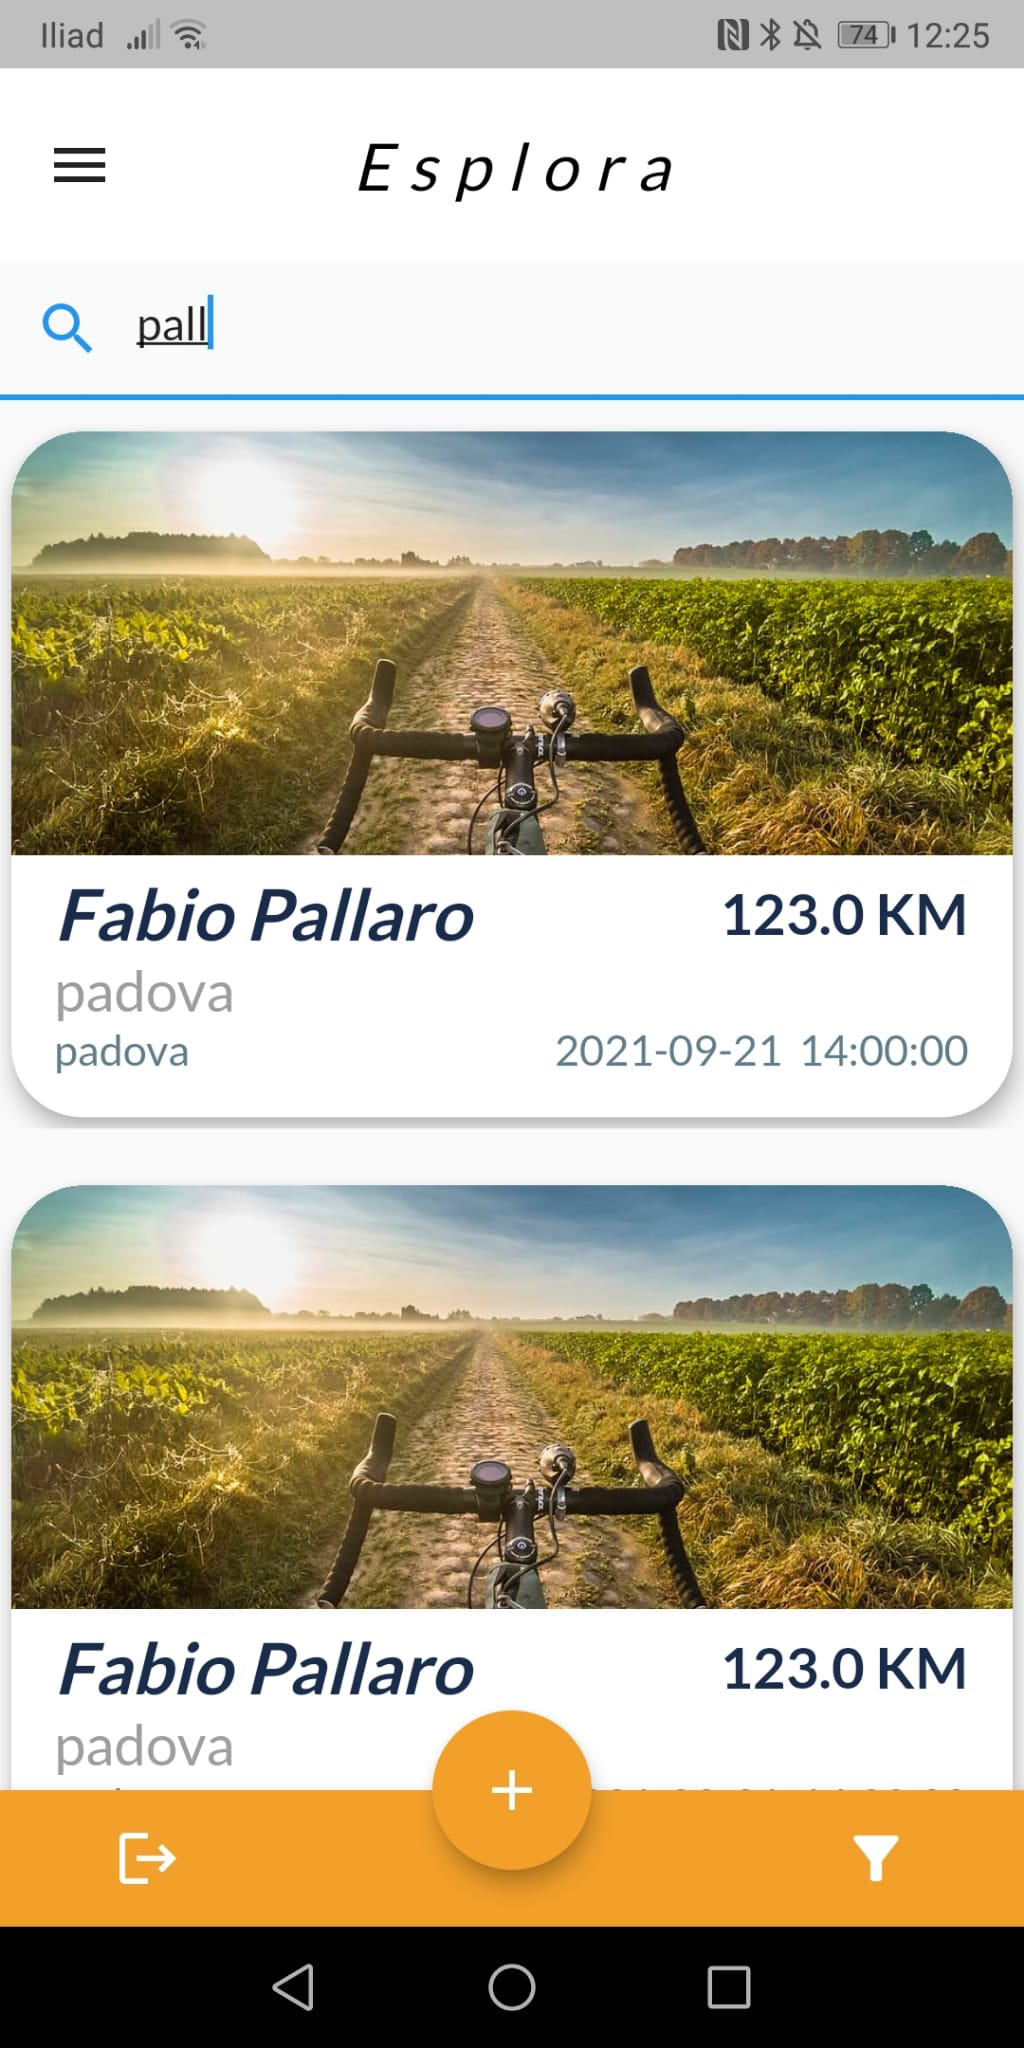
\includegraphics[width=6cm]{immagini/filtrotesto.jpeg}
	\caption{Filtro di ricerca testo}
	\label{fig:Filtro di ricerca testo}
\end{figure}

\newpage

\subsection{Campi obbligatori e pagina modifica e crea}
All'interno di questa pagina sono stati tolti tutti i campi obbligatori non necessari.\\
Per fare ciò sono stati tolti tutti i validator non necessari nel file \textit{pianifica\_screen.dart} e lasciato gli altri validator con le apposite funzioni.\\
Inoltre all'interno di questa pagina sono stati aggiustati i campi degli orari che nella funzione \textit{selezionaOra()} tornava sempre i minuti attuali.\\
Per rendere all'utente più comprensibile il salvataggio è stato sostituita l'icona di salvataggio con l'icona \textit{Icon(Icons.save)}.\\

\begin{figure}[htbp]	
	\centering
	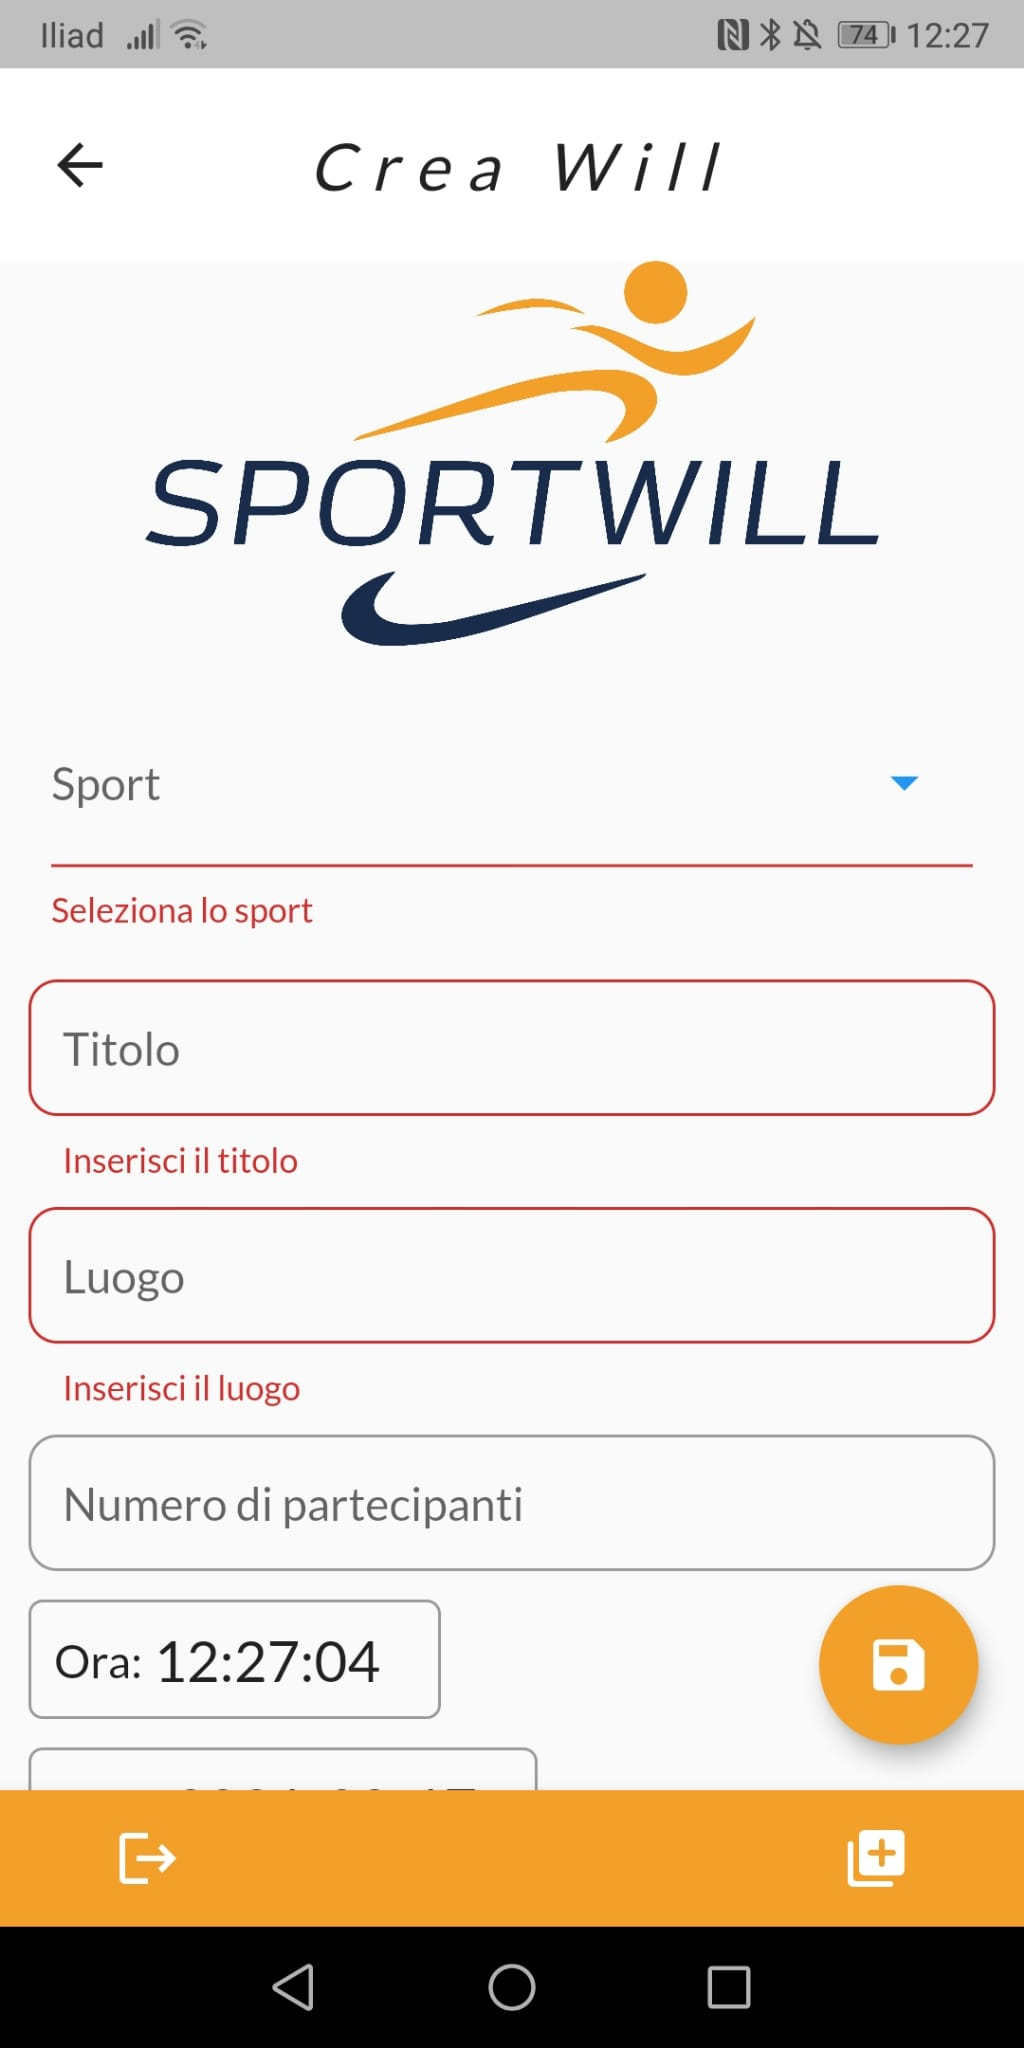
\includegraphics[width=6cm]{immagini/modifica.jpeg}
	\caption{Campi obbligatori}
	\label{fig:Campi obbligatori}
\end{figure}

\newpage

\subsection{Colori}
All'interno dei vari file sono stati cambiati diversi colori in modo che venissero utilizzati principalmente quelli dell'applicazione, ovvero il bianco e l'arancione.\\

\begin{figure}[htbp]	
	\centering
	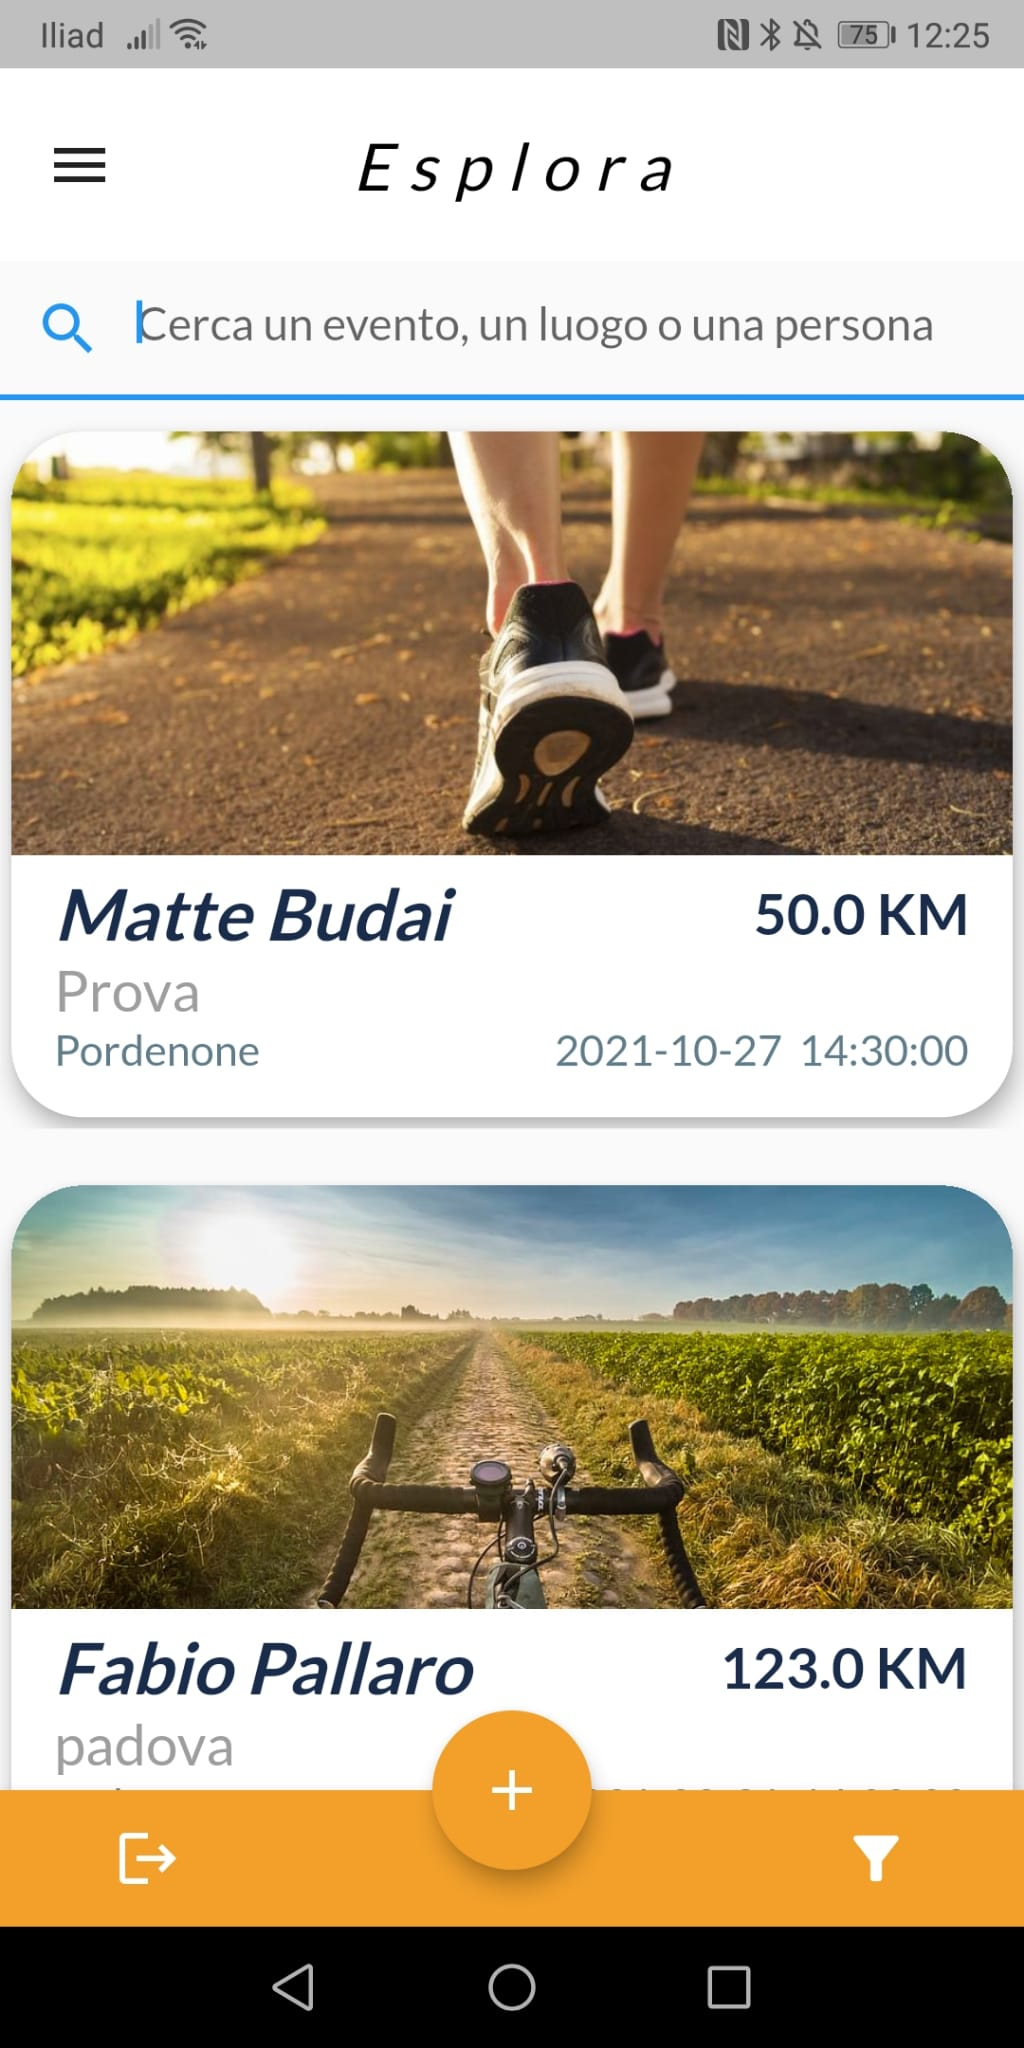
\includegraphics[width=6cm]{immagini/colori.jpeg}
	\caption{Colori}
	\label{fig:Colori}
\end{figure}


\subsection{Eliminazione, Modifica e Aggiunta di un'attività}
In seguito alle modifiche di vari campi sono state sistemate le pagine di eliminazione, modifica e aggiunta di un'attività con nuovi valori e formati in modo che venissero rispettate le richieste del backend.\\
In particolar modo sono stati sistemati i valori che riguardavano la data e l'orario con i nuovi formati richiesti e la lunghezza e il numero di partecipanti che richiedevano un double e un intero.

\newpage

\subsection{Mappa percorso}
Per gestire la mappa sono stati creati due providers:
\begin{itemize}
	\item location.dart: che è il modello e contiene tutti i dati che riguardano una posizione;
	\item locations.dart: che permette di chiamare il backend per ottenere i vari valori da visualizzare nella mappa.
\end{itemize}
La mappa viene creata nel file \textit{dettaglio\_screen.dart} e viene mostrata solo se c'è almeno una posizione per l'attività selezionata.\\
Per visualizzare la mappa viene usato Leaflet e viene creato un array con tutte le posizioni che vengono poi disegnate sulla mappa mettendo i marker alla prima posizione e all'ultima in ordine temporale.\\

\begin{figure}[htbp]	
	\centering
	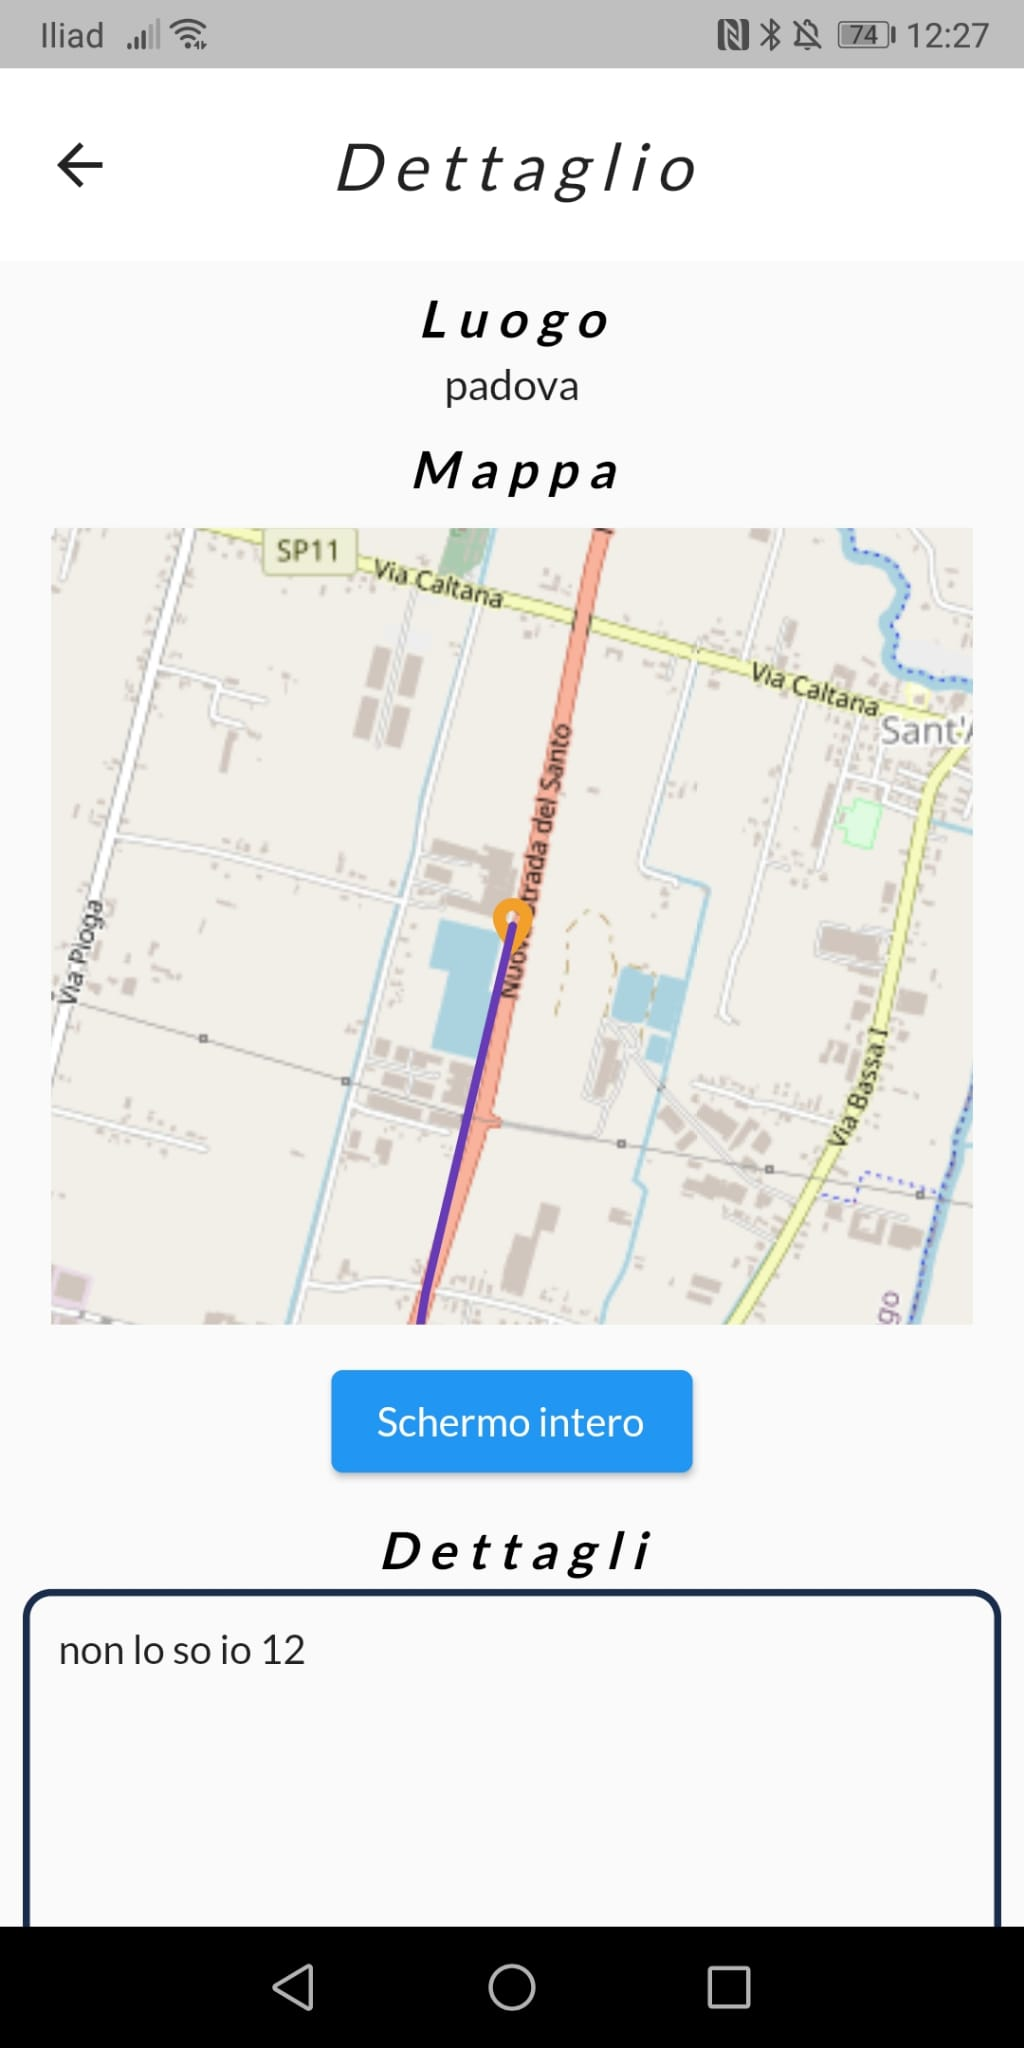
\includegraphics[width=6cm]{immagini/mappa.jpeg}
	\caption{Mappa percorso}
	\label{fig:Mappa percorso}
\end{figure}

\newpage

\subsection{Aggiornamento automatico mappa}
Per fare in modo che la mappa si aggiornasse in modo automatico è stato inserito un Timer che ogni 30 secondi va a chiamare la funzione che ritorna tutte le posizioni di quell'attività.\\
Per evitare che il Timer venisse ricostruito ogni volta è stato usato un valore booleano che permette la costruzione del Timer solo la prima volta.\\

\begin{figure}[htbp]	
	\centering
	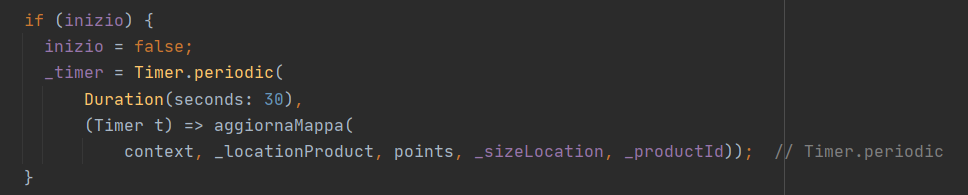
\includegraphics[width=14cm]{immagini/automatico.png}
	\caption{Aggiornamento automatico mappa}
	\label{fig:Aggiornamento automatico mappa}
\end{figure}

\newpage

\subsection{Mappa schermo intero}
Per fare in modo che la mappa fosse più utilizzabile dall'utente è stata creata la possibilità di vederla a schermo intero.
Per fare ciò è stato usato un valore booleano, ovvero \textit{ingradisci} inizialmente uguale a false, che se settato a true permetteva di vedere nello schermo solo la mappa.\\
Cliccando sul bottone \textit{schermo intero} veniva settato questo valore a true e veniva ricostruita la pagina invece premendo sull'icona con la croce veniva settato il valore a false ricostruendo sempre la pagina.\\

\begin{figure}[htbp]	
	\centering
	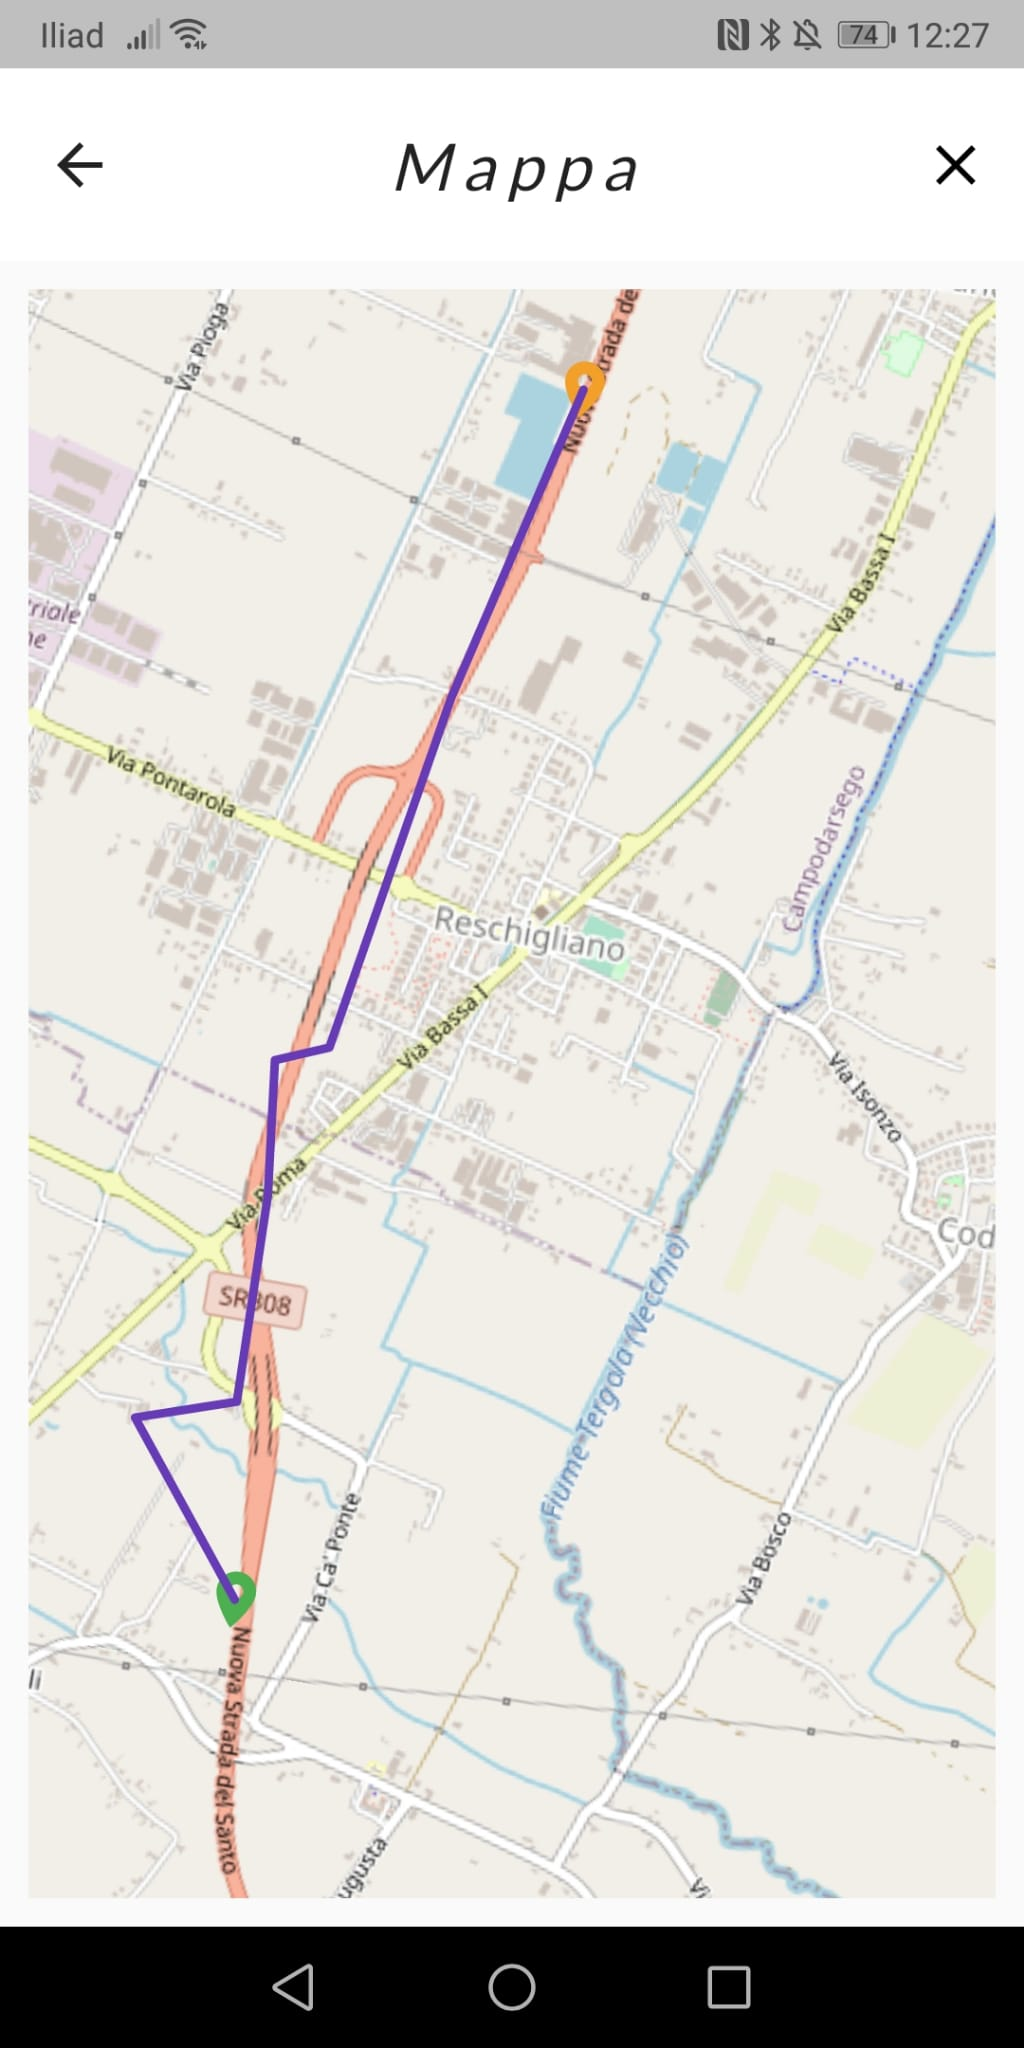
\includegraphics[width=6cm]{immagini/mappaintero.jpeg}
	\caption{Mappa schermo intero}
	\label{fig:Mappa schermo intero}
\end{figure}

\newpage

\subsection{Filtro avanzato di ricerca attività}
Per creare il filtro avanzato è stata creata una funzione \textit{showFilterMenu()} nel file \textit{uscite\_overview\_screen.dart} che contiene una \textit{showDialog}.\\
Per aprire il menù dei filtri bisognerà premere sull'icona dei filtri situata in basso a destra.\\
All'interno di questo menu è possibile filtrare le attività in base allo sport, alla data e se si tratta di tue attività.\\
Per applicare i vari filtri, ovvero quando si preme sull'icona check, è stata utilizzato un booleano che ricostruisce la pagina  con filtro uguale a true e va a chiamare nel provider \textit{uscite.dart} la funzione \textit{findBySporteData} in base ai valori messi nel filtro.\\
L'icona con la croce, una volta premuta, setta il valore del filtro a false e ricostruisce la pagina chiudendo la showdialog dei filtri e cancellando i filtri precedentemente applicati.\\
Per poter capire se abbiamo applicato i filtri basterà guardare se l'icona dei filtri ha il colore verde.\\
Invece se non avremo filtri applicati l'icona avrà il solito colore bianco.\\

\begin{figure}[htbp]	
	\centering
	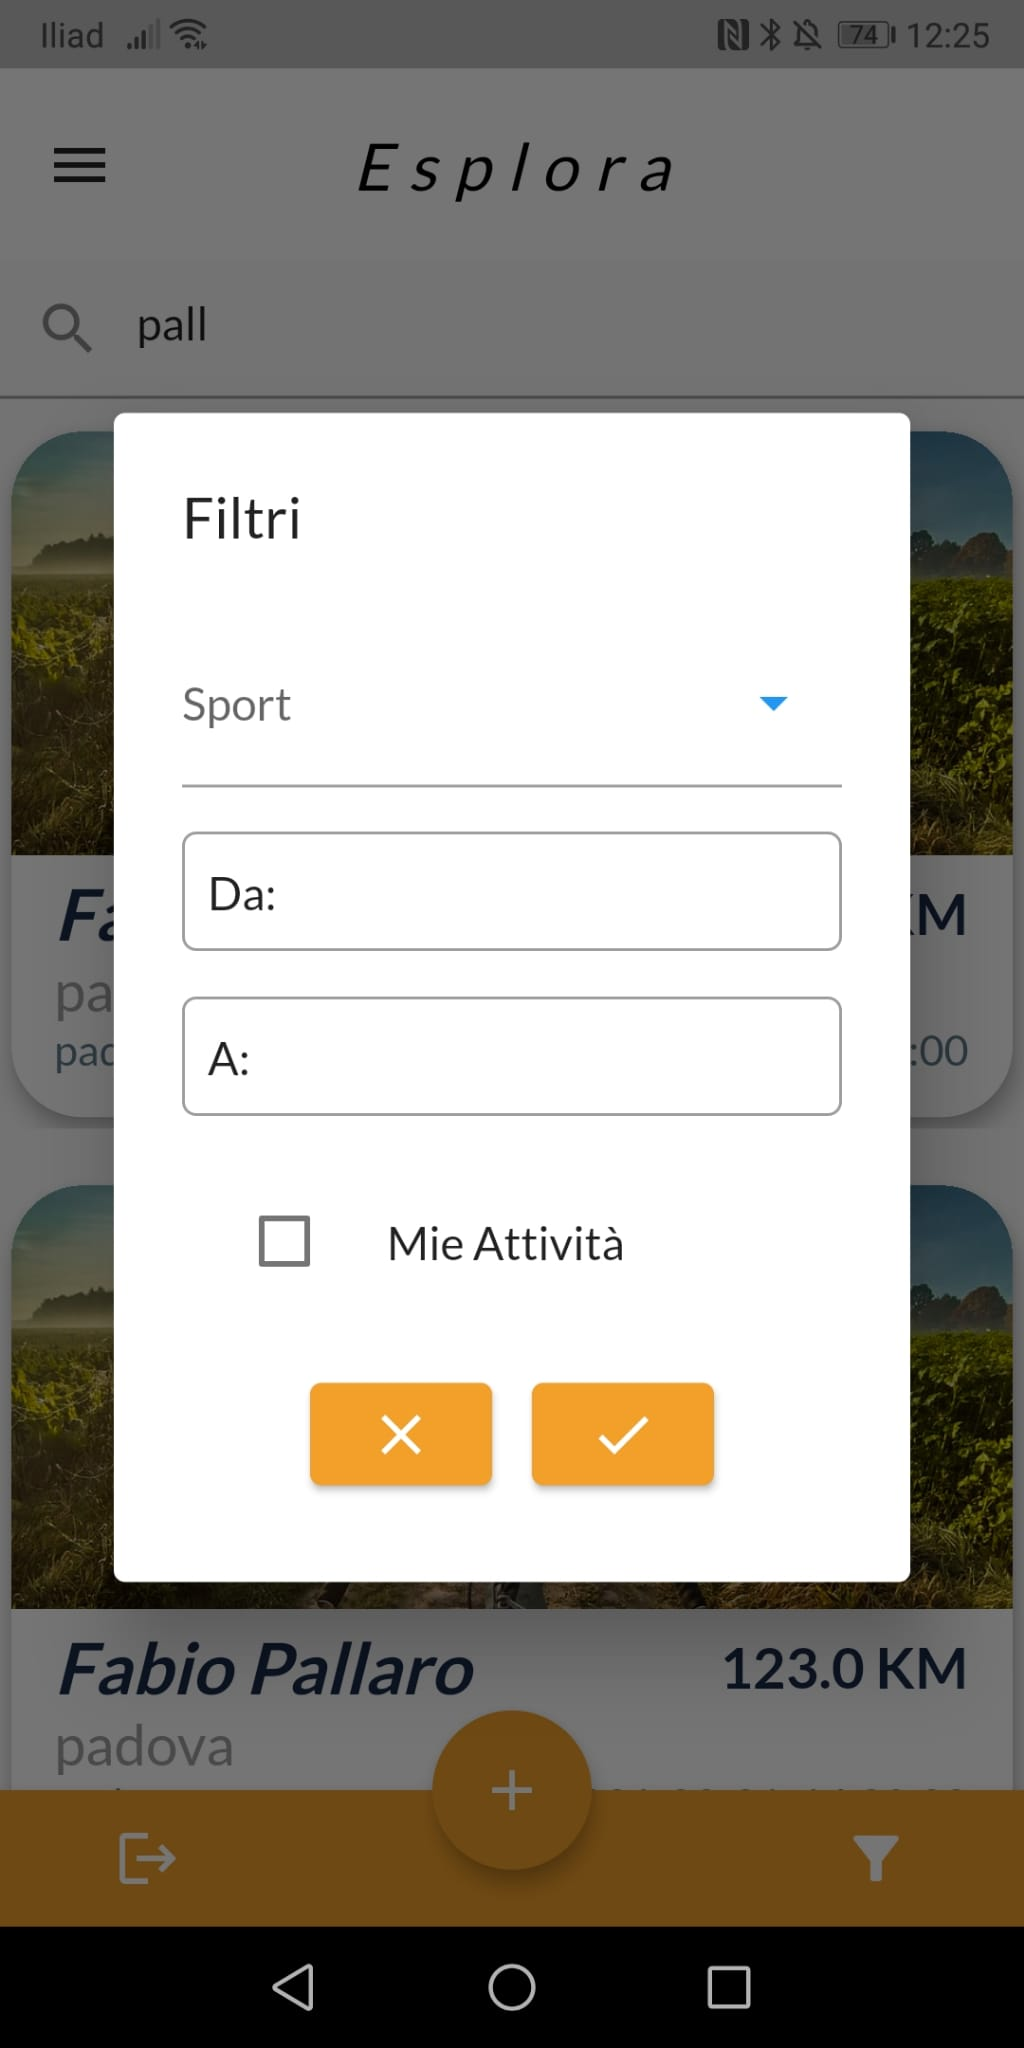
\includegraphics[width=6cm]{immagini/filtroavanzato.jpeg}
	\caption{Filtro avanzato di ricerca attività}
	\label{fig:Filtro avanzato di ricerca attività}
\end{figure}

\newpage

\subsection{Pubblicazione applicazione Play Store}


